\chapter{워터마크 형상}

카멜레온은 기존 화상회의용 워터마크 기술이 가지는 한계를 극복한 워터마크
기술이다. 카멜레온은 회의 호스트 정보 뿐만 아니라 회의 참석자 정보를 추가하여,
회의영상을 녹화하는 참석자가 누구인지 알 수 있다. 또한 워터마크 메시지에 MAC을
삽입하여 메시지의 진위성을 확인 할 수 있다. 카멜레온은 기존 워터마크 기술과
비슷한 방식으로 텍스트를 삽입했고, QR코드를 이용하여 그림 형태 워터마크를
삽입했다. QR코드 워터마크는 회의영상을 실시간으로 캡처하여 QR코드 색을 캡처한
사진의 색과 비슷하게 생성한다. 이를 통해 AI가 QR코드와 회의영상과 구분할 수 없게
했다.

\section{텍스트 워터마크}

텍스트 워터마크는 콘텐츠 이용자가 메시지를 그대로 볼 수 있는 워터마크이다.
텍스트 워터마크를 사용하여 회의 참석자가 회의를 녹화하고 유출하면 안된다는
경각심을 가질 수 있다. 따라서 기존 영상 화상회의 서비스가 제공하는 워터마크
기술과 비슷하게 텍스트 워터마크를 삽입했다. 그러나 기존 워터마크는 유출자를
식별하지 못하고, 진위성을 판별할 수 없다. 카멜레온은 기존 텍스트 워터마크
메시지에 유출자 정보와 MAC을 삽입하여, 이 문제를 해결했다. 그리고 AI 제거 도구가
텍스트 워터마크를 지우지 못하는 경우를 고려하여 텍스트의 형태를 설정했다.

\subsection*{메시지 구성}

% 어떤 메시지를 삽입했는가?
카멜레온은 워터마크 메시지로 주의 사항, 호스트 식별 정보, 참석자 식별 정보, 현재
시간, 메시지 인증 코드를 사용한다.

\begin{itemize}
    \item \textbf{주의사항.} 텍스트 워터마크는 회의 참석자에게 하고 싶은 말을
    전달할 수 있다. 참석자에게 화상회의를 녹화하지 말라는 주의사항을 전달하여,
    실수로 녹화하는 일이 없도록 한다. 카멜레온은 "Do Not Copy!"를 메시지로
    삽입했으며, 다른 메시지를 사용할 수 있다.
    \item \textbf{호스트 식별정보.} 화상회의 영상의 소유권은 호스트에게 있다.
    회의 영상이 유출됐을 때, 워터마크로부터 호스트 정보를 얻어 영상 소유권이
    호스트에게 있음을 증명할 수 있다. 
    \item \textbf{참석자 식별정보.} 회의 참석자 식별 정보는 각 참석자 PC마다
    서로 다르다. 회의영상이 유출되었을 때, 참석자 식별 정보를 확인하여 어느
    참석자의 PC에서 유출되었는지 확인할 수 있다.
    \item \textbf{현재시간.} 회의를 진행하고 있는 현재 시간을 워터마크 삽입하여,
    유출된 회의가 언제 진행한 회의인지 알 수 있다. 현재 시간은 실시간으로
    갱신하여 새로운 메시지를 삽입한다.
    \item \textbf{메시지 인증 코드.} 메시지 인증 코드(이하 MAC)는 데이터가
    변조되었는지 검증 할 수 있도록 데이터 뒤에 덧붙이는 코드이다. 코드를 생성할
    때는 호스트의 키를 사용하여, 호스트만 데이터 변조 여부를 알 수 있다.
    카멜레온은 호스트 식별 정보, 참석자 식별 정보, 현재 시간 세 개의 메시지에
    대해 MAC값을 계산한다. 회의영상이 유출되면, 호스트는 자신의 키를 사용하여
    워터마크 메시지의 MAC을 계산하고, 워터마크로 삽입된 MAC과 같은지 확인하여
    메시지 진위성을 확인한다.
\end{itemize}

그림 \ref{fig:text_wm}은 텍스트 워터마크를 삽입한 회의영상 사진 일부이다.
주의사항으로 ``Do Not Copy!"를 보여주어, 회의 참석자들에게 회의영상을 복사하지
말라고 권고한다. Alice는 회의 호스트, Bob은 회의 참석자 중 한명의 식별정보이다.
Bob이 아닌 다른 참석자의 회의 영상에서는 해당 부분이 다른 정보로 나타난다.
그리고 현재 시간 2024...가 나타나 있으며, 밑에는 Alice-Bob-현재시간에 대한 MAC
값을 삽입했다. 사용한 키는 호스트 Alice의 키이며, 여기서는 `chameleon'를 키로
사용하고, 알고리즘은 SHA256을 사용했다.
\begin{figure}[ht]
    \vspace{10pt}
    \centering
    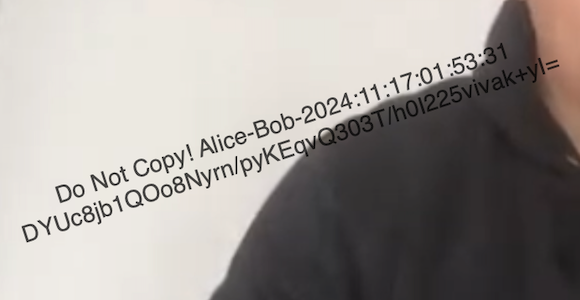
\includegraphics[width=0.6\textwidth]{imgs/text_wm.png}  % 이미지 파일명 (여기서는 예시 이미지 사용)
    \caption{텍스트 워터마크 구성}
    \label{fig:text_wm}
\end{figure} 


\subsection*{삽입 방식}

% 텍스트의 형태는 어떻게 되는가?
다양한 형태로 텍스트를 삽입해본 결과, 텍스트 워터마크가 회의영상 속 텍스트와
유사하면, AI 제거 도구는 텍스트 워터마크를 지우지 못한다. 혹은 지우더라도 원본을
크게 훼손한다. 따라서 폰트, 글자 크기, 글자 색 등을 결정할 때, 화상회의 화면에
주로 보이는 텍스트와 유사하게 구성했다. 일반적으로 화상회의에서는 문서를
보여주거나 발표자료를 보여주기 때문에, 이 때 자주 사용하는 글자 형태에 맞췄다.
그러나 이렇게 텍스트 워터마크를 삽입하면, 회의 참석자 또한 워터마크와 문서 속
텍스트와 구분하기 어려워 회의 참여가 불편할 수 있다. 따라서 텍스트 워터마크를
기울여 문서 내 글과 구분했다.

% 화면에 어떻게 삽입하는가?
텍스트 워터마크는 많이 삽입할수록 추출할 가능성이 높다. 화면을 가리지
않으려고 일부에만 워터마크를 삽입할 경우, 유출자는 해당 부분을 자르고 영상을
유출시킬 수 있다. 따라서 카멜레온은 텍스트 워터마크를 화면 전체에 골고루
삽입했다. 또한 카멜레온은 워터마크에 애니메이션 효과를 줬다. AI 워터마크 제거
도구는 화면의 특정 영역을 선택해 워터마크를 지우는 기능이 있다. 워터마크의
위치가 고정되면, 선택 영역이 좁아져 원본을 크게 훼손하지 않고 워터마크를 지울 수
있다. 워터마크 위치를 옮기면 선택 영역이 넓어진다. 또한 워터마크가 움직이기
때문에 화면을 계속 가리지 않는다. 


\section{QR 코드 워터마크}

QR코드는 2차원 매트릭스 바코드의 일종이다. QR 코드는 오류정정기법을 사용해,
코드를 일부 훼손하더라도 그 안에 있는 메시지를 유지할 수 있다. 워터마크는
콘텐츠가 시간이 지남에 따라 열화되면서 훼손될 수 있고, 유출자에 의해 훼손될 수도
있다. QR 코드를 이용하여 워터마크를 삽입하면, 이러한 훼손에도 워터마크 내
메시지를 추출할 수 있다. 카멜레온은 QR 코드의 특성을 활용하기 위해,
QR코드로 워터마크를 삽입한다.


\subsection*{메시지 구성}


QR코드 워터마크가 담는 메시지는 텍스트 워터마크와 동일하다. 주의사항을
제외한 참여자 식별정보, 유출자 식별정보, 현재시간, MAC값을 담는다. 다만, 4
가지 정보를 하나의 QR코드에 담지 않고, MAC값은 다른 QR코드로 만들어, 두 개의
QR코드를 만든다. QR코드 크기는 78px로, 44 바이트 메시지를 담을 수 있다.

그림 \ref{fig:qr_wm}는 카멜레온이  QR코드 워터마크를 삽입한 영상 일부이다. 왼쪽
위 QR코드와 오른쪽 QR 코드가 다른 것을 알 수 있는데, 각각 식별정보와 현재시간을
담은 QR코드, MAC값을 담은 QR코드이다.
\begin{figure}[ht]
    \vspace{10pt}
    \centering
    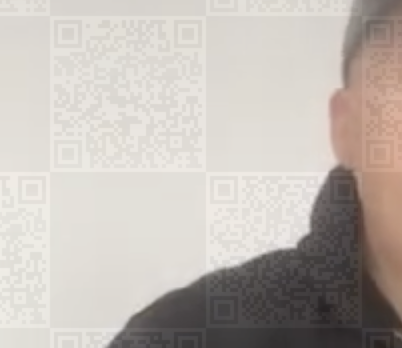
\includegraphics[width=0.4\textwidth]{imgs/qr_wm.png}
    \caption{QR코드 워터마크 구성}
    \label{fig:qr_wm}
\end{figure} 

\subsection*{삽입 방식}

카멜레온은 QR코드를 삽입 하기 전 QR 코드 색상을 결정한다. 색상은 화상회의 화면에
의존한다. 화상회의 화면을 캡처한 후 QR 코드를 삽입할 위치에 해당하는 픽셀의 평균
RGB를 계산한다. 이 값을 QR코드 색으로 결정한다. 그림 \ref{fig:qr_wm_color}는
QR코드 워터마크 색상 변경 방식을 그림으로 표현한 것이다.
\begin{figure}[ht]
    \vspace{10pt}
    \centering
    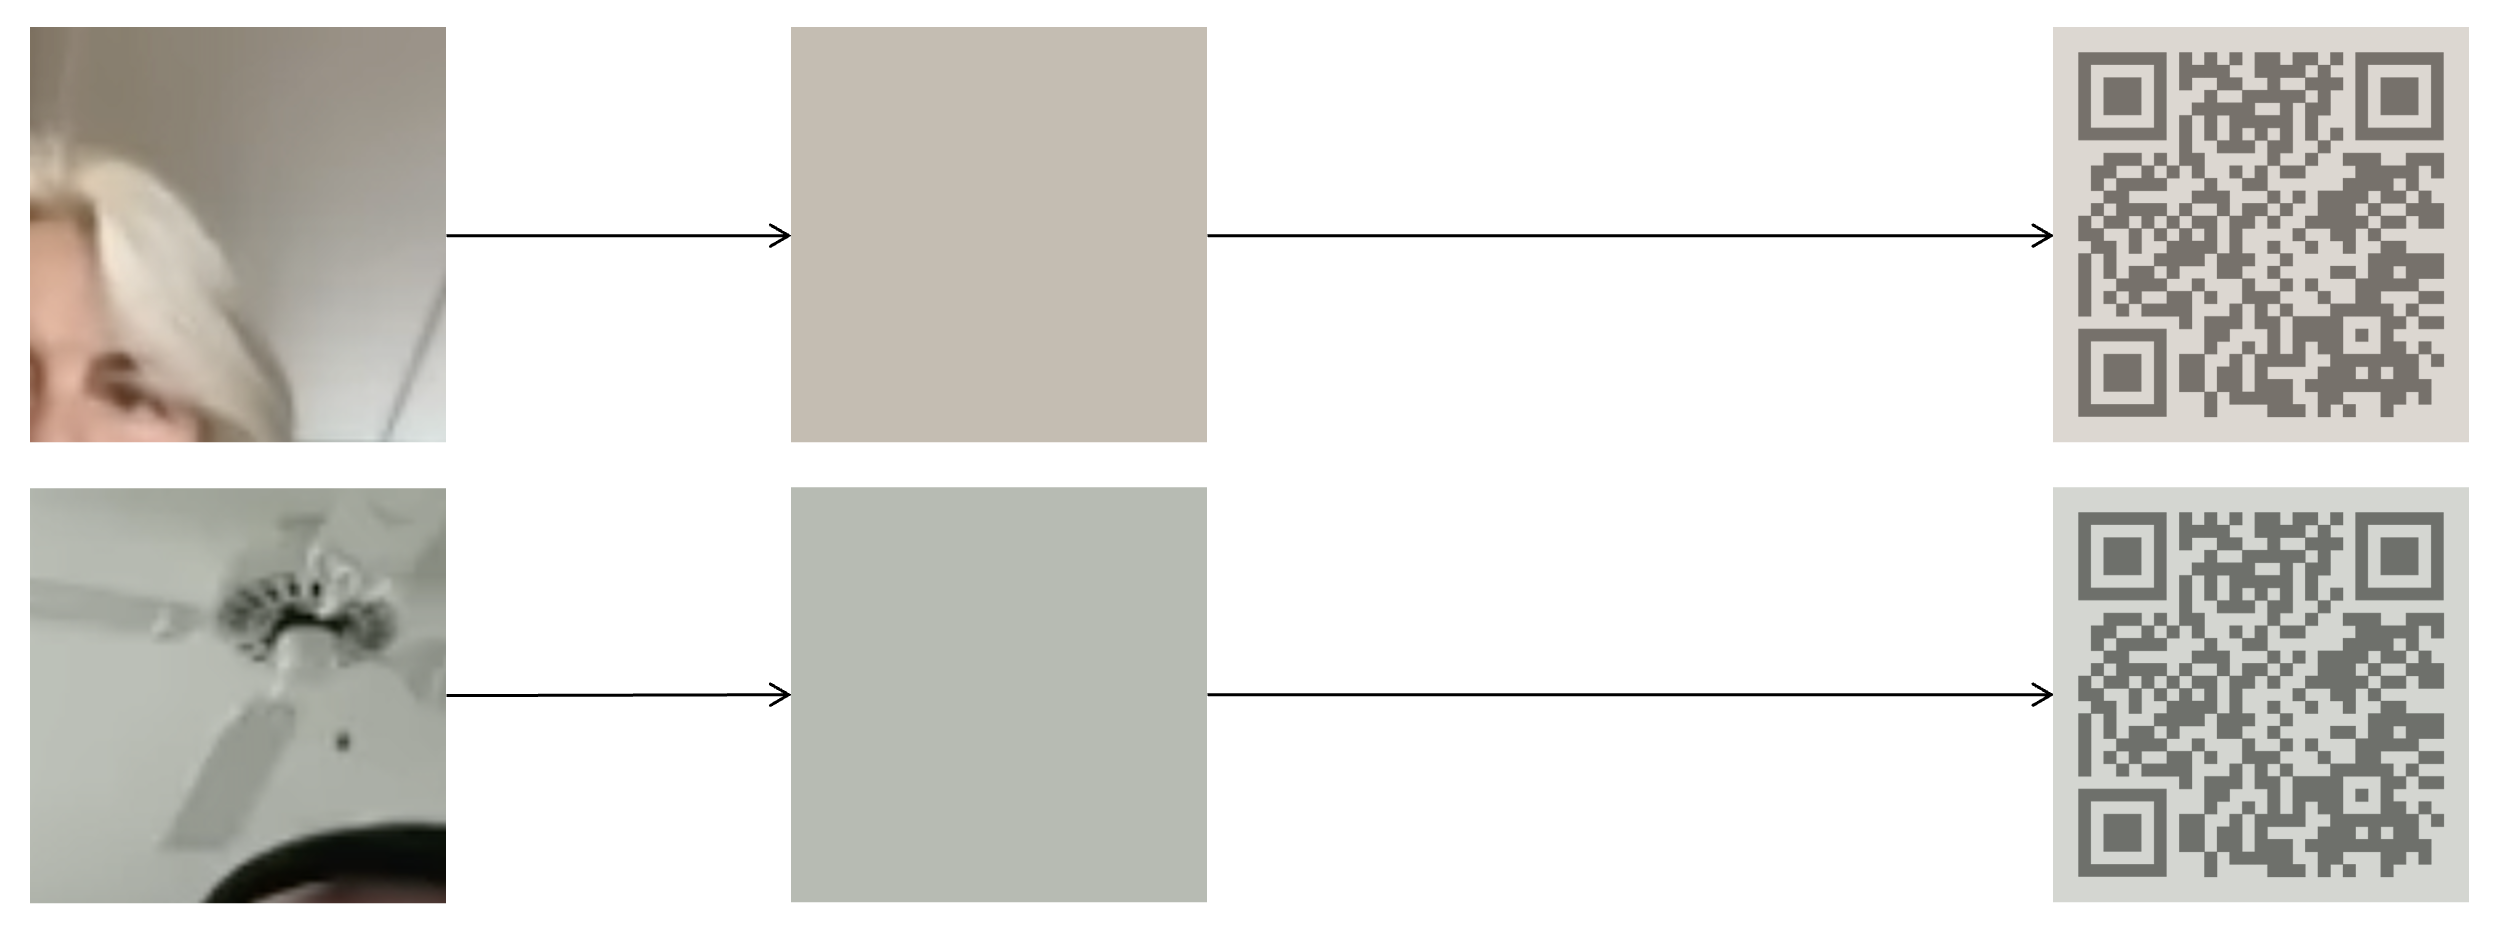
\includegraphics[width=0.8\textwidth]{imgs/qr_wm_color.png}
    \caption{QR코드 워터마크 색상 변경 방식}
    \label{fig:qr_wm_color}
\end{figure} 

이 방식은 두 가지 기대효과를 가진다. AI 워터마크 제거 도구는 QR코드 워터마크를
지울 수 있다. QR코드 색상을 화상회의 화면 색과 유사하게 변경하면 AI는 QR코드 워터마크와 화상회의
영상을 구분하지 못하기를 구분할 수 있다. 실험 결과, QR코드를 흑백으로 삽입했을
때보다, 색상을 비슷하게 만들어 삽입했을 때 AI는 덜 훼손하는 것을 확인했다.
그리고 QR코드를 화면 전체에 투사하면 회의 참석자는 QR코드에 의해 화면을 잘 보지 못할 수
있다. 따라서 QR코드 워터마크의 투명도를 높여 참석자가 회의영상을 시청할 때
불편함 을 줄일 수 있다. QR코드 색상을 뒷 배경 색과 비슷하게 만들면, QR코드의
투명도가 높아지는 효과를 줄 수 있다.

카멜레온은 두 종류의 QR코드를 화면에 체크무늬 형태로 출력한다. QR코드를 화면에 가득 채우면
회의에 방해가 될 수 있고, 향후에 비어있는 공간을 활용하여 다른 형태의
워터마크를 삽입할 수 있게 했다. 